\chapter{Theoretical background}
\label{chapter:theoreticalbackground}
User interface design is a thoroughly studied discipline with strong roots in psychology. In the 1980s \acrshort{gui} development exploded due to better hardware\cite{myers1998brief}. This meant that traditional user interfaces had to be redesigned to accommodate to the graphical features of the modern computer. Chapter~\ref{chapter:introduction} described the issues visually impaired users experienced with this new method of interaction. Section~\ref{section:apacheisis} will describe what Apache Isis entails. Furthermore, section~\ref{section:previouswork} expands on existing efforts to improve usability for the visually impaired. Finally, section~\ref{section:pitfallsinuserinterfaceadaptation} briefly addresses some pitfalls when a user interface is adapted to a new form.

\section{Apache Isis}
\label{section:apacheisis}
Picking a framework for developing web applications can be a tedious process. There are dozens of frameworks for Java alone, with the oldest and most adopted one being Spring\cite{Sprin96:online}. The vast majority of these frameworks are based on the \textit{\acrlong{mvc}} (\acrshort{mvc}) pattern, where the view displays information to the user, the controller processes interaction between the user and the view, and the model contains the information and business logic that manipulates this information\cite{leff2001web}. The relations between the components are depicted in figure~\ref{figure:mvc}.

\begin{figure}[h]
	\center
	\include*{figures/mvc}
	\caption{Interaction between the components of an MVC application}
	\label{figure:mvc}
\end{figure}

While the \acrshort{mvc} pattern itself has a lot of advantages, it has received criticism in the context of web development. The concept of separating business logic from presentation logic is often not adhered to in web applications, resulting in controllers that are contaminated with logic that should live in the model\cite{Fulfi2:online}. Trygve Reenskaug, who introduced the \acrshort{mvc} pattern while working at the Xerox Palo Alto Research Center in 1978, concluded that true \acrshort{mvc}-based applications were hard to achieve\cite{reenskaug2007programming}:

\begin{displayquote}
\textit{"The conventional wisdom in the group was that objects should be visible and tangible, thus bridging the gap between the human brain and the abstract data within the computer. This simple and powerful idea failed ... because users were used to seeing objects from different perspectives. The visible and tangible object would get very complex if it should be able to show itself and be manipulated in many different ways."}
\end{displayquote}

\subsection{Domain-driven development}
\label{subsection:domaindrivendevelopment}
Even though Reenskaug did not consider the \acrshort{mvc} pattern to be successful, the philosophy of displaying information in a manner that feels natural to humans is still a very valid one. Many methodologies have been developed in an attempt to capture this philosophy, of which \textit{\acrlong{ddd}} (\acrshort{ddd}) is a well-known example. Conceived by Eric Evans in 2004, \acrshort{ddd} strives to streamline and align the domain experts (the business experts) and the technical experts (the developers). Through the process of clearly defining which terms to use for specific concepts and ensuring that both parties understand what they mean, a \textit{ubiquitous language} is formed, and information asymmetry can be avoided\cite{evans2004domain}. The \textit{domain model} is then built solely with terms in the ubiquitous language. The key to success in \acrshort{ddd} is then to apply model-driven development; by developing the software while strictly adhering to the specified domain model, all stakeholders are able to comprehend the content of the software. If the domain model proves to be insufficient to implement a new feature, the stakeholders should work together to extend the ubiquitous language in order for the domain model to become complete again. This creates a bidirectional relationship between the domain model and the code: when the domain model changes, so does the code and vice versa.

\subsection{Naked Objects pattern}
\label{subsection:nakedobjectspattern}
One of the frustrations often expressed regarding \acrshort{ddd} is that while the ubiquitous language combined with the derived domain model may very well tackle the problem of goal diversion, it also increases overhead greatly. Consider figure~\ref{figure:applicationlayers}, in which the domain model is represented in the business logic layer. As the domain model is refined over the course of time, any changes to the domain model must be reflected in the code. This means that any modifications to the domain model will have to be applied to the other layers, too.

\begin{figure}[h]
	\center
	\include*{figures/applicationlayers}
	\caption{The main application layers in \acrshort{ddd}}
	\label{figure:applicationlayers}
\end{figure}

To address this issue, Richard Pawson designed the \textit{\acrlong{no}} (\acrshort{no}) pattern, based on three core concepts\cite{pawson2002naked}:
\begin{enumerate}
	\item Business logic should only reside in domain objects\footnote{A domain object is an entity that holds relevant data, in order to transfer the data between the application layers.}
	
	\item The user interface is an exact representation of the domain objects, and thus is an object-oriented user interface
	
	\item The user interface is derived completely and fully automatically from the domain objects through reflection\footnote{Reflection is a language's ability to inspect and dynamically call classes, methods, attributes, etc. at runtime.}
\end{enumerate}

These three concepts combined provide a means of developing software that robustly follows the philosophy of \acrshort{ddd}. The first two concepts ensure that the software implements the domain model and prevents the use of technical language. The application, whether prototypal or deployed, will feel familiar to the stakeholders and developers alike. The third concept is not necessarily related to \acrshort{ddd}, but does take away the burden of developing the presentation layer, thus placing the focus on the business logic (i.e. the domain model). Due to these characteristics, Reenskaug states in the foreword of Pawson's thesis that the \acrshort{no} pattern could be seen as an important extension and implementation of the original \acrshort{mvc} pattern.

\subsection{Java Framework}
\label{subsection:javaframework}
Apache Isis is a framework written in Java that implements the \acrshort{no} pattern. The core strength of the framework is that behaviour, which would normally be defined in controllers in classical \acrshort{mvc} applications, is automatically generated by reflection. A major benefit of this feature is that prototyping is greatly simplified; the business logic is virtually all that needs to be programmed, and the framework does the rest. This means that project managers, product owners, and other parties involved can be presented with working prototypes rather than charts and specifications. It furthermore relieves developers from wasting precious time on coding the visible part of an application - code which often has limited reusability in a later stage of development.

This does not, however, imply that Apache Isis is merely useful for prototyping. The automatically generated interface is perfectly suitable for a lot of business-oriented applications. Estatio\cite{Estat40:online}, an estate management application built on Apache Isis which is commissioned by a listed real estate investment firm, makes use of the standard wicket viewer. In case a given application demands a bespoke user interface, it can be designed to use the \acrshort{rest} API which ships with Apache Isis and which will be used to implement our interface.

Due to the underlying \acrshort{no} paradigm that the user interface is derived from the domain objects, Apache Isis is exceptionally suitable for this research project. All of the information that dictates what is visible to the user can be found in the code that describes the functionality of the software. Thus, we are able to develop a new user interface that retrieves everything it needs from what the developers have written, regardless of the interface they intend to use.

\noindent
\begin{figure}
\begin{minipage}{.5\textwidth}
\begin{javacode}
@DomainObject
public class SimpleObject implements Comparable<SimpleObject> {
    public TranslatableString title() {
        return TranslatableString.tr("Object: {name}", "name", getName());
    }

    @javax.jdo.annotations.Column(allowsNull="false")
    @Property
    @Getter @Setter
    private String name;

    public TranslatableString validateName(final String name) {
        return name != null && name.contains("!") ?
            TranslatableString.tr("Exclamation mark is not allowed"): null;
    }
}
\end{javacode}
\end{minipage}
\begin{minipage}{.5\textwidth}
	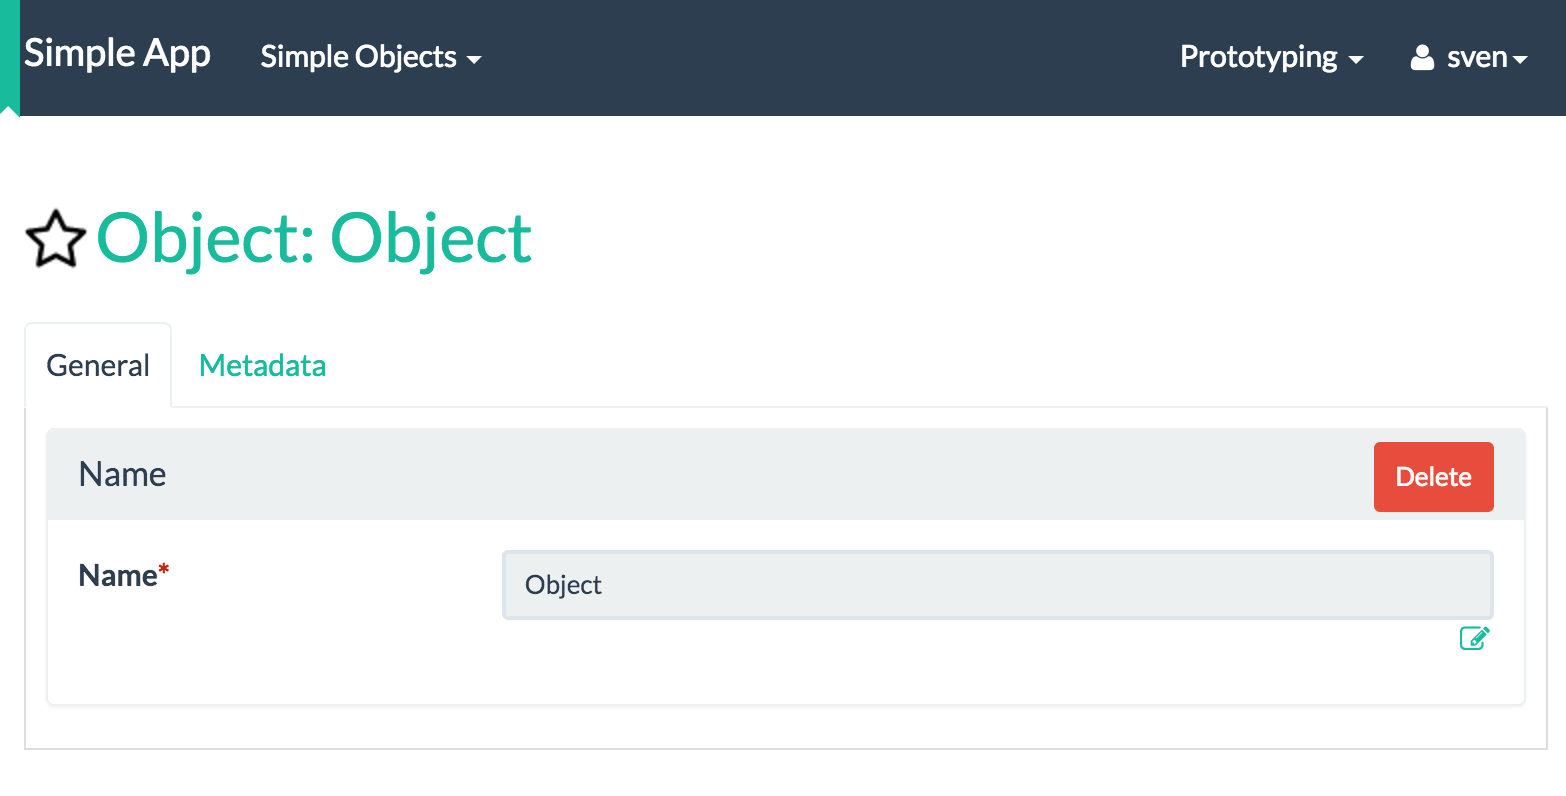
\includegraphics[width=\textwidth]{figures/simpleobjectui}
\end{minipage}
\caption{A very simple example of how the user interface is derived from code}
\end{figure}

\section{Previous work}
\label{section:previouswork}
User interfaces make use of at least one of the traditional human senses to convey information, be it vision, hearing or another sense. It is evident that \acrshortpl{gui} are mainly based on exploiting human vision. As visually impaired people lack this sense, they have to interact with software through what remains: the auditory, somatic, gustatory, and olfactory senses. The latter two senses are relatively unexplored in terms of human-computer interaction. While there have been developments such as 'smicons', representing icons through odour\cite{kaye2001symbolic}, and a display that represents rudimentary information through scents sprayed in the direction of the nose\cite{yanagida2004projection}, it has proven difficult to employ these senses in a practical manner. The main reason is that smell and taste are chemical rather than physical sensations and thus a lot harder to synthesise, let alone synthesise accurately\cite{kortum2008hci}. Therefore, effectively only two senses remain available: the auditory and somatic senses.

Exploiting the hearing sense is a good way of making software usable for a larger audience, as it only requires a form of audio output to function and virtually all modern devices either have built-in speakers or a headphone jack. Most auditory user interfaces synthesise text to speech and use auditory icons for basic operations, such as the sound of crumpling paper on a delete operation\cite{mynatt1995transforming}. While this is regarded as one of the easiest ways of increasing accessibility of software, it still leaves a portion of the auditory sense unused, as it does not take advantage of spatial sound. Research has shown that basic elements of interfaces, such as menus, can be displayed very effectively in a spatial setting\cite{frauenberger2004spatial}.

Software can also interact with the somatic sense through haptic feedback. Tactile feedback is a form of haptic feedback that relies on the sensation of touch, vibration, and pressure. Visually impaired people who have learned braille can take advantage of output devices called braille terminals combined with screen reader software, which translates text on the screen to braille. This does not, however, offer practical support for graphical elements. With the advent of mobile technology, research in the field of tactile user interfaces has increased. The majority of these mobile devices have touch screens and vibrating motors, allowing gesture-based input and haptic feedback\cite{kane2008slide, yatani2009semfeel}.

\section{Pitfalls in user interface adaptation}
\label{section:pitfallsinuserinterfaceadaptation}
The concept of universally accessible user interfaces has gained a lot of traction since the widespread adoption of \acrshortpl{gui}. It has proven difficult, however, to adapt an interface in such a way that it becomes both universally accessible and maintainable. The foremost shortcoming of adapting an existing user interface is that it is mainly an a posteriori change, thus any future changes to the software will require modifications to all existing user interfaces. Another issue is that it may be very difficult or even impossible to adapt certain functionality due to the constraints of the new interface\cite{emiliani2000adaptations}. Furthermore, a lack of standardisation can increase the required amount of labour to an extent that it is no longer feasible to perform the adaptation\cite{moore1993issues}. Currently, it is generally accepted that it is more convenient and successful to take a proactive approach of making design choices with universal accessibility in mind, as opposed to a reactive approach of adapting an existing design\cite{savidis2004unified}. However, considering this is not within the scope of this research, we will not address this in detail.